\documentclass{article}

\usepackage[utf8]{inputenc}
\usepackage{amsmath}
\usepackage[uniquename=init,firstinits,backend=bibtex,sorting=none]{biblatex}
\usepackage{calc}
\usepackage{color}
\usepackage{gensymb}
\usepackage{graphicx}
\usepackage{listings}
\usepackage[numbered,framed]{mcode}
\usepackage[space]{grffile}
%% hyperref manual advises loading this package last
\usepackage{hyperref}
\hypersetup{colorlinks=true,linkcolor=blue,citecolor=blue,breaklinks=true}

\definecolor{gray}{rgb}{0.9,0.9,0.9}

\lstloadlanguages{Matlab}
\lstset{basicstyle=\small,breaklines=true,frame=single,float,columns=fullflexible,numbers=left,stepnumber=2,backgroundcolor=\color{gray}}

\newcommand{\reals}{\mathbf R}

\newcommand{\FIXME}[1]{\\\fbox{FIXME: #1}\\}

\title{An Algorithmic Introduction to Lagrangian Coherent Structures}

\author{Kristjan Onu \and Florian Huhn \and George Haller}

\addbibresource{main}

\begin{document}

\numberwithin{equation}{section}
\numberwithin{figure}{section}
\numberwithin{lstlisting}{section}
\numberwithin{table}{section}

\maketitle

\tableofcontents

\abstract{
We give a practical introduction to Lagrangian coherent structures (LCSs.) The article reviews recent results in variational LCS theory, presents algorithms to detect LCSs in two dimensional time dependent flows, and demonstrates a LCS computational engine called LCS Tool using examples.
}

\section{Introduction}

LCSs are used in fluid dynamics to capture essential flow features and thereby simplify the description of fluid flows. More specifically, LCSs have been particularly well adapted to analyze two dimensional finite time turbulent flows. LCSs capture dominant transport barriers, repelling and attracting structures and LCSs are used to identify vortex boundaries.

LCSs have been used to analyse oceanic and atmospheric flows, biological applications\parencite{wilson09:_lagran_reynol,tallapragada11:_lagran}, aeronautics\parencite{tang10:_accur_lagran_hong_kong_inter_airpor} and mechanical systems\parencite{hadjighasem13:_detec_kam}.

The finite-time Lyapunov exponent (FTLE) gives a mathematical definition for LCSs. Although the FTLE has been applied to a variety a situations, it is possible to find examples where it fails to identify LCSs correctly, giving false positives and false negatives\parencite{haller11:_lagran_coher_struc,norgard12:_secon_lagran_coher_struc}. To remedy these problems, variational principles have been used to present new approaches to identifying LCSs\parencite{haller11:_lagran_coher_struc,farazmand12:_comput_lagran,haller12:_geodes_theor_trans_barrier_two_dimen_flows,farazmand13:_attrac_lagran,haller13:_coher_lagran}.

This article presents an algorithmic introduction LCSs using a computational engine for LCSs called LCS Tool\footnote{LCS Tool is free MATLAB software available for download at: \url{https://github.com/jeixav/LCS-Tool}}.

LCS Tool is a library of functions that perform the computations to identify LCSs in two dimensional finite time flows. LCS Tool aims to initiate scientists to LCSs. Existing LCS software programs are:
\begin{itemize}
\item \emph{MANGEN}\parencite{lekien03:_time}, calculates stability manifolds adaptively in two dimensional finite time velocity fields. Includes a graphical user interface and uses MPI for parallel calculations.
\item \emph{LCS MATLAB Kit}\parencite{dabiri09:_lmk} calculates the FTLE from velocity datasets. Includes a graphical user interface.
\item \emph{Newman}\parencite{toit10:_trans} calculates the FTLE in $N$ dimensions. Assists ridge extraction of FTLE fields. Supports analytic and dataset defined velocity definitions.
\item \emph{FlowVC}\parencite{shadden10:_flowvc} is a general purpose LCS platform for two and three dimensional datasets. Parallel calculations are supported with Open\-MP, CUDA and OpenCL.
\end{itemize}
These packages are based on the FTLE; the objective of this article and LCS Tool is to replace FTLE methods.

\section{Theory}

The fluid flows considered are defined in two dimensions by a velocity field:
\begin{align*}
\dot{\boldsymbol x} = \boldsymbol v(\boldsymbol x,t), && \boldsymbol x \in U \subset \reals^2, && t \in [t_-,t_+].
\end{align*}
Integration yields the flow map, defined between an initial time $t_0$ and a final time $t$ within $[t_-,t_+]$:
\[
F_{t_0}^t(\boldsymbol x_0) := \boldsymbol x(t,t_0,\boldsymbol x_0).
\]
The time interval used to detect LCSs is left as a choice; it can be the complete interval for which the flow is defined, or data is available, or it can be a chosen subset.

The right Cauchy-Green strain tensor measures Lagrangian strain in the velocity field and is defined:
\[
C_{t_0}^t(\boldsymbol x_0) = \left[\nabla F_{t_0}^t(\boldsymbol x_0)\right]^T \nabla F_{t_0}^t(\boldsymbol x_0).
\]
The eigenvalues of the Cauchy-Green strain tensor are denoted by $\lambda_{1,2}$ and the eigenvectors by $\boldsymbol \xi_{1,2}$. The eigenvalues satisfy $0 < \lambda_1 \leq \lambda_2$ and the eigenvectors satisfy $\boldsymbol \xi_1 \perp \boldsymbol \xi_2$.

We find coherent Lagrangian vortices by considering strain, as was done in~\textcite{haller13:_coher_lagran}. To summarise the results in that publication, we examine closed curves $\gamma$ and $O(\epsilon)$ neighbourhoods or ``belts'' around them. For most $\gamma$, neighbouring belts of $O(\epsilon)$ exhibit strain variability of $O(\epsilon)$. Curves that form coherent Lagrangian vortices are exceptional however and display no observable variability in their average strain within $O(\epsilon)$ neighbourhoods.

The mathematical identification of a coherent Lagrangian vortex para\-metrises a curve $\gamma$ by $\boldsymbol r(s)$ with $s \in [0,\sigma]$ at time $t_0$. The length of a tangent vector $\boldsymbol r'(s)$ is $l_{t_0}(s)$. The advected curve $F_{t_0}^t(\gamma)$ has a tangent vector $(\text{d}/\text{d}s) F_{t_0}^t(\boldsymbol r(s))$ and a length we denote by $l_t(s)$. The two tangent lengths are calculated:
\begin{gather*}
l_{t_0} = \sqrt{\langle \boldsymbol r'(s), \boldsymbol r'(s) \rangle},\\
l_t = \sqrt{\langle \boldsymbol r'(s), C_{t_0}^t(\boldsymbol r(s)) \boldsymbol r'(s) \rangle},\\
\end{gather*}
where $\langle \cdot, \cdot \rangle$ denotes the Euclidean inner product.
The average tangential strain along $\gamma$ is:
\[
Q(\gamma) = \frac{1}{\sigma} \int_0^\sigma \frac{l_t(s)}{l_{t_0}(s)}\text{d}s.
\]

Coherent Lagrangian vortices are associated with the strain tensor
\[
E_\lambda(\boldsymbol x_0) = \frac12 [C_{t_0}^t(\boldsymbol x_0) - \lambda^2 I]
\]
and curves uniformly stretched by the same factor $\lambda$ when advected by the flow from time $t_0$ to $t$ are closed trajectories of one of two explicit 
differential equations: 
\begin{equation}
\boldsymbol r' = \boldsymbol \eta_\pm(\boldsymbol r),
\label{e:etafields}
\end{equation}
where
\[
\boldsymbol \eta_\pm = \sqrt{\frac{\lambda_2 - \lambda^2}{\lambda_2 - \lambda_1}} \boldsymbol \xi_1 \pm \sqrt{\frac{\lambda^2 - \lambda_1}{\lambda_2 - \lambda_1}} \boldsymbol \xi_2.
\]
In subsequent sections $\lambda = 1$ always.

We find hyperbolic LCSs from a variational approach based on shear, as presented in~\textcite{farazmand13:_shearless}. The Lagrangian shear is calculated:
\[
p(s) = \frac{\langle \boldsymbol r'(s), D(\boldsymbol r(s)) \boldsymbol r'(s)\rangle}{\sqrt{\langle \boldsymbol r'(s), C(\boldsymbol r(s)) \boldsymbol r'(s)\rangle \langle \boldsymbol r'(s), \boldsymbol r'(s)\rangle}}
\]
where
\[
D(\boldsymbol x_0) = \frac12[C(\boldsymbol x_0) \Omega - \Omega C(\boldsymbol x_0)], \quad \Omega = \begin{pmatrix}0&-1\\1&0\end{pmatrix}.
\]
The average Lagrangian shear along a curve $\gamma$ over the time interval $[t_0,t]$ is:
\[
P(\gamma) = \frac{1}{\sigma} \int_0^\sigma p(s) \text{d}s.
\]

Similarly to Lagrangian vortices, exceptional hyperbolic curves without shear in $O(\epsilon)$ neighbourhoods are null-geodesics of the Lorentzian metric
\[
g(\boldsymbol u, \boldsymbol v) = \langle \boldsymbol u, D(\boldsymbol x_0) \boldsymbol v \rangle.
\]
Repelling LCSs are obtained as solutions of the strainline differential equation:
\[
\boldsymbol r' = \boldsymbol \xi_1(\boldsymbol r),
\]
and attracting LCSs are obtained as a solution of the stretchline differential equation:
\[
\boldsymbol r' = \boldsymbol \xi_2(\boldsymbol r).
\]

\section{Methods}

This section presents the numerical methods used to compute Lagrangian coherent structures. In other words, the algorithms that constitute LCS Tool are presented.

\subsection{The Cauchy-Green strain tensor}

To obtain Lagrangian coherent structures the Cauchy-Green strain tensor must be calculated first. More specifically, the eigenvalues and eigenvectors of the Cauchy-Green strain tensor are needed. The function associated with this calculation in LCS Tool is \texttt{eig\_cgStrain}. The main steps of this function are enumerated in Table~\ref{t:Cauchy-Green algorithm}.

\begin{table}
\begin{enumerate}
\item Setup a Cartesian grid and auxiliary grid in the (rectangular) domain of the flow.
\item Integrate the flow velocity equations at each grid point and auxiliary grid point. This yields the flow map, $F_{t_0}^t(\boldsymbol x_0)$.
\item Use finite differences to approximate the derivative of the flow map, $D F_{t_0}^t(\boldsymbol x_0)$.
\item Compute the Cauchy-Green strain tensor, $C_{t_0}^t = \left(D F_{t_0}^t\right)^T D F_{t_0}^t$ and its eigenvalues, $\lambda_{1,2}$ and eigenvectors, $\xi_{1,2}$.
\end{enumerate}
\caption{Algorithm used to calculate the Cauchy-Green strain tensor eigenvalues and eigenvectors.}
\label{t:Cauchy-Green algorithm}
\end{table}

We setup a Cartesian grid according to user-defined resolutions. We can find the optimal resolution by an iterative procedure in which we start with a low resolution and double it until convergence of LCSs is observed visually. A resolution of about 500 grid point along the longest axis usually gives good results. Furthermore an auxiliary grid is setup. This is illustrated in Figure~\ref{f:main and auxiliary grids}. The improvements the auxiliary grid yields compared to using only the main grid were reported in \textcite{farazmand12:_comput_lagran}. Experience indicates that optimal results are obtained when the auxiliary grid spacing is between 1 and 10\% of the main grid spacing.

\begin{figure}
\begin{center}
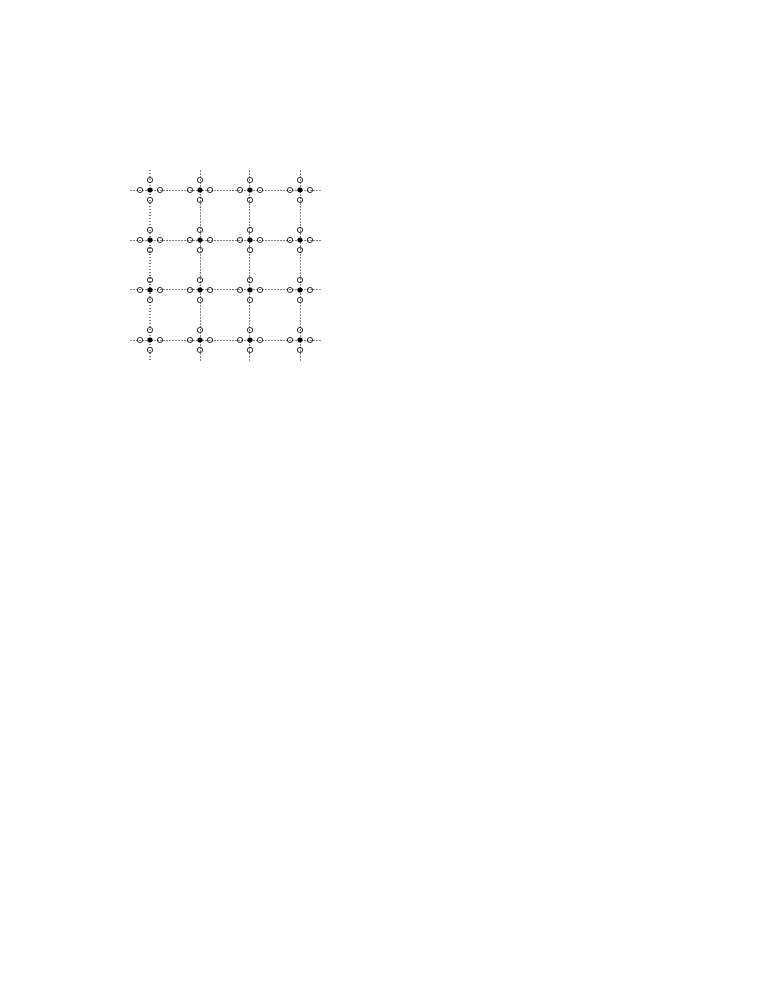
\includegraphics[width=\textwidth]{graphics/main_aux_grids}
\end{center}
\caption{Illustration of main and auxiliary grid used to compute the Cauchy-Green strain. Solid circles are main grid points and hollow circles are auxiliary grid points.}
\label{f:main and auxiliary grids}
\end{figure}

The function \texttt{eig\_cgStrain} provides the option to calculate the eigenvector from the auxiliary grid, but the eigenvalues from the main grid. We have found that for flows defined analytically the eigenvalues should be calculated from the main grid whereas for the flows defined by datasets, using the auxiliary grid gives better results.

As stated, typically we set the main grid resolution of the Cauchy-Green strain tensor to around 500 grid points. For a square domain, this implies the velocity equations must be integrated, after including 4 auxiliary grid points around every main grid point, at 1.25 million grid points. The ``natural'' way to perform these integration calculations would be to solve a two dimensional first-order ODE system at every grid point and iterate over every grid point within a for-loop. With 1.25 million grid points this calculation can take an excessively long time. To alleviate this problem, we solve the flow equations in a vector form where the equations at all grid points are combined into a single system of equation, even though the system of composed of independent blocks of two dimensional first-order ODE systems. MATLAB's \texttt{ode45} function is used to perform the integration and the flow integration typically takes five to ten minutes with default error tolerances. The drawback of vector form integration is its memory requirements can become excessive at high resolutions, furthermore, writing the velocity function in vector form is more error-prone than the intrinsic two dimensional form.

The Cauchy-Green strain tensor can have singularities (i.e. $C_{t_0}^t(\boldsymbol x_0) = I$). Such points are isolated in general\parencite{delmarcelle94}, therefore no special accommodations for are made in computations for singularities of the Cauchy-Green strain tensor.

\subsubsection{Special case: incompressible velocity fields}

Flows that are incompressible, meaning $\nabla \cdot \boldsymbol v = 0$, satisfy the relation $\lambda_1(\boldsymbol x_0) \lambda_2(\boldsymbol x_0) = 1, \forall \: \boldsymbol x_0 \: \in \: U$\parencite{arnold78:_mathem}. This gives the possibility of imposing incompressibility when calculating the eigenvalues of the Cauchy-Green strain tensor by first calculating $\lambda_2$ and then setting $\lambda_1(\boldsymbol x_0) = 1/\lambda_2(\boldsymbol x_0)$. This procedure should be applied carefully since by changing $\lambda_1$ but not $\xi_1$, the error in satisfying the eigenvalue equation for the Cauchy-Green strain tensor may increase.

At some grid points it may occur that $\lambda_2 < 1$ due to numerical integration errors of the flow velocity equations. By setting integration tolerances to smaller values the number of grid points with $\lambda_2 < 1$ can be reduced. Nonetheless, some grid points can be so close to singularities of the Cauchy-Green strain tensor that satisfying $\lambda_2 >= 1$ everywhere could be excessively computationally costly. Therefore the function \texttt{eig\_cgStrain} records the number of points at which incompressibility cannot be imposed and this measure can also help to set appropriate integration tolerances.

\subsubsection{Special case: data-defined velocity fields}

Velocity fields defined by datasets require pre-processing prior to performing the integration that yields the flow map. An interpolation function must be written to enable evaluating the velocity function at arbitrary points in $U$ and at arbitrary times between $t_-$ and $t_+$. MATLAB's interpolation functions can be integrated into the velocity function. As with analytic cases, care should be taken to ensure the interpolation embedded in the flow velocity integration function works correctly when performing integration in vector form.

Beyond the pre-processing needed to obtain the Cauchy-Green strain tensor eigenvalues and eigenvectors, no special manipulations are needed to treat data-defined flow. It may be however, that parameter values giving good results with analytically defined flows need adjustment prior to processing data-defined velocity fields.

\subsection{Shear LCS}

Shear LCSs, or coherent Lagrangian vortices, are closed orbits in the Lagrangian shear vector fields $\boldsymbol \eta_{\pm}$ defined in Equation~\eqref{e:etafields}. Since $\lambda = 1$, the closed curves are non-stretching and area preserving. We find closed orbits by integrating shearlines starting from a Poincare section and evaluating the first return map. A shearline closing onto itself in the starting point is a shear LCS. 

The main steps of the algorithm used to calculate shear LCS are enumerated in Table~\ref{t:Shear LCS algorithm}

\begin{table}
\begin{enumerate}
\item Position Poincare sections in flow domain
\item Calculate Poincare return map
\item Find closed orbits in Poincare return map
\item Identify outermost closed orbit
\end{enumerate}
\caption{Algorithm used to calculate Shear LCS.}
\label{t:Shear LCS algorithm}
\end{table}

The first step is to set the position of Poin\-care sections \texttt{poincare\-Section.endPosition} that are straight lines in regions where closed shearlines are expected. The Poincare section must be oriented in a way that the first endpoint is close to the centre of the expected eddy and the second endpoint is outside the expected eddy region. There is no predetermined procedure for deciding where the Poincare sections should be positioned. Possibilities are an examination of the finite-time Lyapunov exponent field of the flow, or some prior knowledge of where coherent eddies could be expected. Additionally, the number of trajectories launched from the Poincare section \texttt{poincareSection.numPoints} must be defined. A good default value is $100$.

The second step is to integrate the shearlines to obtain the Poincare return map. Integration of shearlines is performed with the $\eta_+$ and $\eta_-$ vector fields defined on the main grid. These vector fields are derived from eigenvalues and eigenvectors as described in~\textcite{farazmand12:_comput_lagran}. The eigenvector fields have orientation discontinuities, therefore the vector field must be locally reoriented for the integration. The algorithm used to perform variable step-size integration in vector fields with orientation discontinuities is enumerated in Table~\ref{t:variable step integration} and illustrated in Figure~\ref{f:variable step integration}. Linear interpolation is used when interpolating $\boldsymbol \eta_\pm$ within a grid element, since using higher order interpolation would necessitate verifying that there are no orientation discontinuities at more than only the four nearest grid points. Detection of orientation discontinuities is achieved by checking the inner product of the vector fields at adjacent grid points. Then, rotations exceeding 90\degree\, are classified as orientation discontinuities and are corrected before linear interpolation. Thus when setting the Cauchy-Green strain tensor main grid resolution, a histogram of eigenvector field rotations may be produced to ensure that all rotations are below 90\degree\, or close to 180\degree.

\begin{table}
\begin{enumerate}
\item Linearly interpolate vector field orientation at initial position
\item At next position, check whether vector field has rotated by over 90\degree, if yes, flip the vector field orientation by 180\degree.
\item Stop integration when shearline returns to Poincare section, or maximum integration length has been reached.
\end{enumerate}
\caption{Algorithm used for variable time step integration of shearlines.}
\label{t:variable step integration}
\end{table}

\begin{figure}
\begin{center}
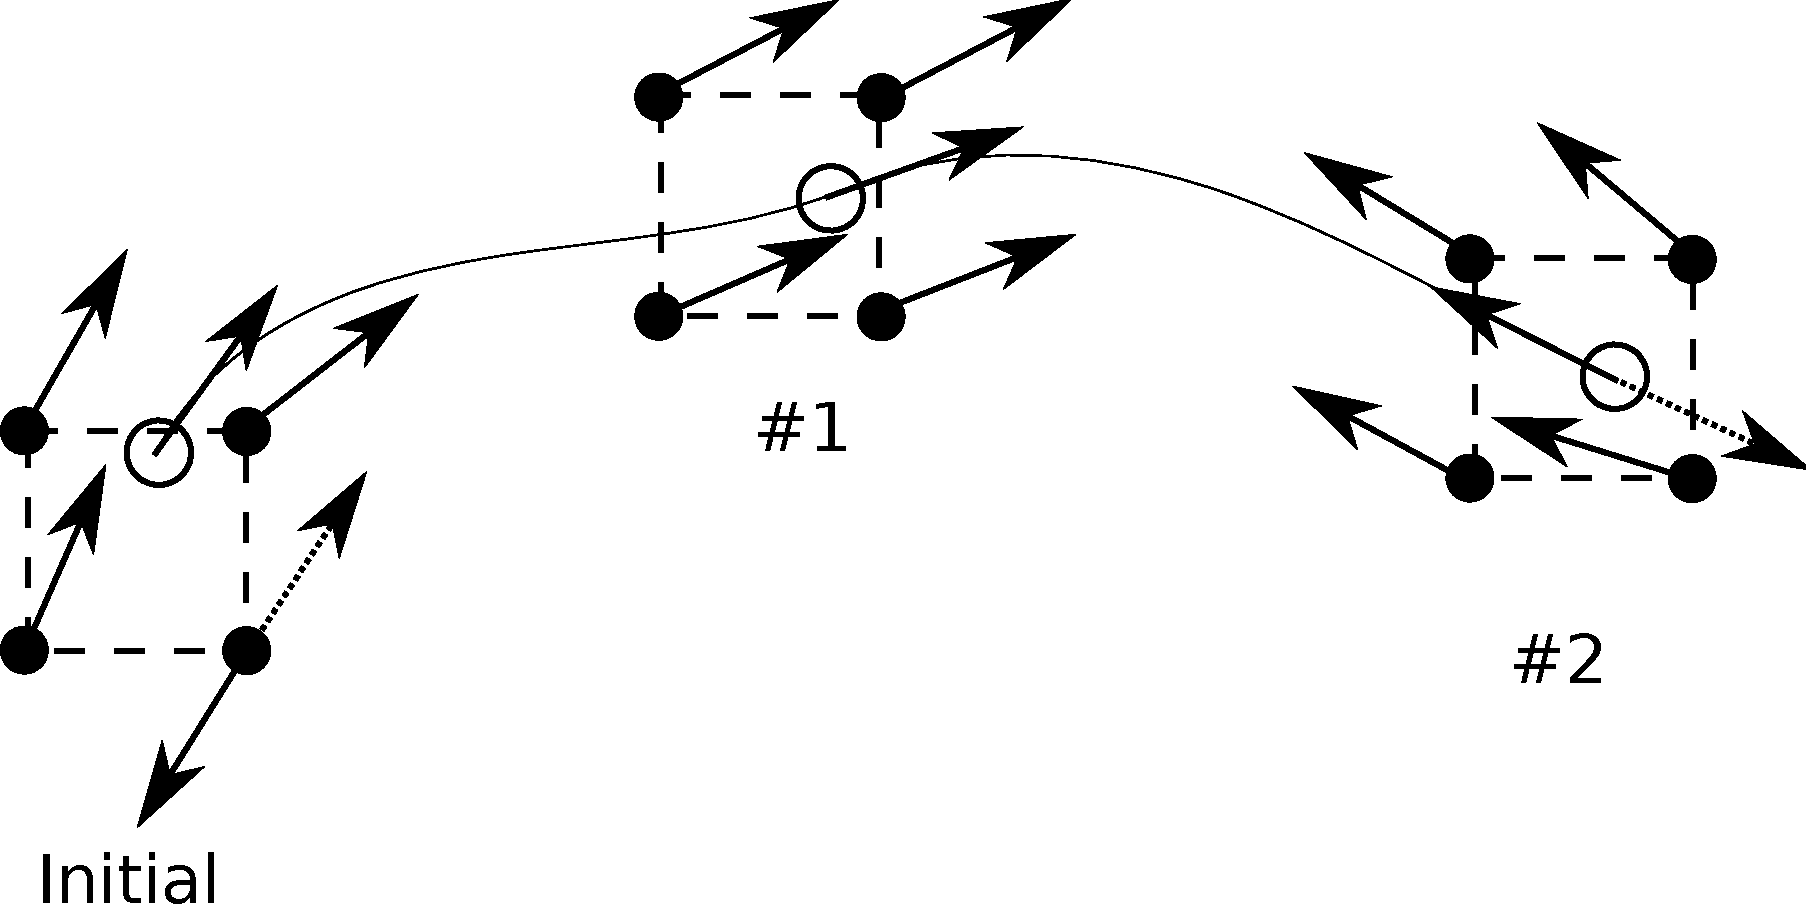
\includegraphics[width=\textwidth]{graphics/variable_step_integration}
\end{center}
\caption{Schematic illustration of shearline variable time step integration. At the initial point, there is an orientation discontinuity at the lower right grid point that must be corrected prior to linear interpolation. At point \#1, no orientation discontinuties are present. At point \#2 the interpolated eigenvector field must be rotated by 180\degree\,to match the orientation at the previous point, \#1.}
\label{f:variable step integration}
\end{figure}

An example of a Poincare return map produced from integration of the $\boldsymbol \eta_\pm$ field is shown in Figure~\ref{f:Poincare return map}. Well behaved orbits will return to the Poincare section and their integration will be stopped using an ODE event detection function. Some orbits may however deviate far from the Poincare section and their integration could take inordinately long. To prevent this behaviour, a maximum orbit length, \texttt{poincareSection.\-orbit\-MaxLength}, is specified. In practice, viewing the Poincare section as the radius of a circle and setting the maximum shearline integration length to twice the circumference gives acceptable results. In Figure~\ref{f:Poincare return map}, circle markers indicate closed orbit positions. Closed orbits exist where the Poincare return map is zero. The function \texttt{poincare\_closed\_orbit} performs the computations. In Figure~\ref{f:Poincare return map} not all zero crossings have circles. This is because a threshold parameter, \texttt{dThresh} whose default value is 1\% of the length of the Poincare section, is used to discard those zero crossings that appear in regions with high numerical noise. The position of each detected zero crossing is refined by iteratively bisecting the interval of the zero crossing. If after a predetermined number of iterations, \texttt{nBisection} whose default value is five, the two points around the zero crossing have absolute values of more \texttt{dThresh}, the zero crossing is discarded. In the Figure, discarded zero crossings are seen where $0 < s < 0.05$. Once all closed shearline orbits have been located, the outermost orbit of every Poincare section is deemed a shear LCS.

\begin{figure}
\begin{center}
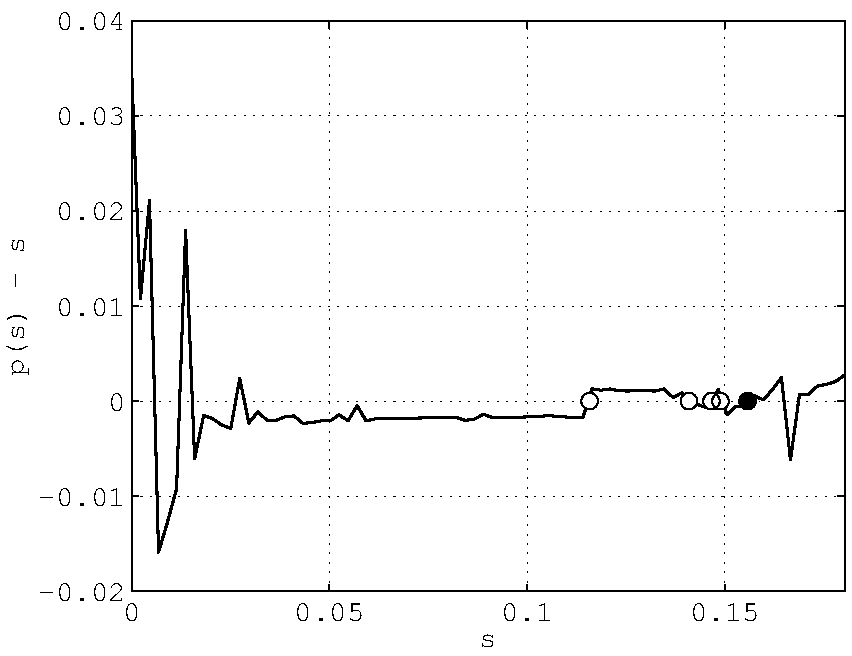
\includegraphics[width=\textwidth]{graphics/double_gyre/poincare_return_map}
\end{center}
\caption{Example of a Poincare return map obtained for shear LCS. Circle markers indicate closed orbit positions. The filled circle indicates the outermost closed orbit and shear LCS.}
\label{f:Poincare return map}
\end{figure}

\subsection{Hyperbolic LCS}

The main steps of the algorithm used to calculate hyperbolic LCS are enumerated in Table~\ref{t:Hyperbolic LCS algorithm}

\begin{table}
\begin{enumerate}
\item Define a local maximisation distance.
\item Find all local maximums of $\lambda_2$ on the main grid such that they are maximums within a circle with a radius equal to the local minimisation distance.
\item Define a maximum strainline length
\item Integrate a strainline forward and backward, using the largest $\lambda_2$ local maximum as the initial position. Integrate until the strainline has attained the maximum strainline length, or until it has reached the domain boundary.
\item Flag any remaining local maximums of $\lambda_2$ within the minimisation distance of the strainline as ineligible initial positions for subsequent strainlines
\item Continue integrating strainlines using local maximums of $\lambda_2$ as initial positions until no eligible local maximums of $\lambda_2$ remain.
\item Remove any strainline segment contained within (closed) shear LCS
\end{enumerate}
\caption{Algorithm used to calculate hyperbolic LCS.}
\label{t:Hyperbolic LCS algorithm}
\end{table}

Strainlines are integrated from local maximums of $\lambda_2$ on the main grid. A local maximisation distance is defined. This distance is set between two and five grid points since it represents the number of grid points over which the Cauchy-Green strain tensor is susceptible to numerical noise from integration. Thus the local maximisation distance is expected to be a function of variable time step integration tolerances. A record is made of all grid points where $\lambda_2$ is maximum within a circle whose radius equals the defined maximisation distance. Then the first strainline is integrated from the largest of all the local maximums forward and backward in time. Similarly to shearlines, this integration must take into account eigenvector field orientation discontinuities. Prior to initiating strainline integration, a maximum length is defined. Strainlines are then integrated until reaching the domain boundary or the maximum length. The maximum length may be seen as safety factor to prevent highly sinuous strainlines leading to inordinately long computations; the maximum length should be set such that most strainline stop at the domain boundary. Once a strainline position has been calculated, local maximums of $\lambda_2$ within the minimisation distance are flagged as ineligible initial positions for subsequent strainlines. After the first strainline has been obtained and any ineligible local maximums of $\lambda_2$ have been flagged the next strainline is integrated. The process continues until all eligible local maximums of $\lambda_2$ have been used to initialise strainline integration. Finally any strainline segment contained within (closed) shear LCS are removed. These calculations are performed by the functions \texttt{seed\_curves\_from\_lambda\_max} and \texttt{remove\_strain\_in\_shear}.

Note that once a strainline integration has begun, it may progress so as to be within the local minimisation distance of an existing strainline. In other words, the local minimisation distance controls where strainlines begin, but not where they stop.

\section{Examples}

\subsection{The double gyre}

The double gyre is a model for a pattern observed in geophysical flows\parencite{shadden05:_defin_lagran_lyapun}. The velocity equations are:
\begin{equation}
\begin{split}
\dot x = -\pi A \sin[\pi f(x,t)] \cos(\pi y)\\
\dot y = \pi A \cos[\pi f(x,t)] \sin(\pi y) \frac{\partial f(x,t)}{\partial x}\\
f(x,t) = \epsilon \sin(\omega t) x^2 + [1 - 2 \epsilon \sin(\omega t)] x
\end{split}
\label{e:double gyre derivative equations}
\end{equation}
The MATLAB function corresponding to these equations is given in Listing~\ref{l:double gyre derivative} and shows how to specify a derivative function that supports vector form integration.

\begin{lstlisting}[caption={Double gyre derivative function corresponding to Equations~\ref{e:double gyre derivative equations}.},label=l:double gyre derivative]
function derivative_ = derivative(t,x,epsilon,amplitude,omega)

idx1 = 1:2:numel(x)-1;
idx2 = 2:2:numel(x);

a = epsilon*sin(omega*t);
b = 1 - 2*epsilon*sin(omega*t);
forcing = a*x(idx1).^2 + b*x(idx1);

derivative_ = nan(size(x));

derivative_(idx1) = -pi*amplitude*sin(pi*forcing).*cos(pi*x(idx2));
derivative_(idx2) = pi*amplitude*cos(pi*forcing).*sin(pi*x(idx2)).*(2*a*x(idx1) + b);
\end{lstlisting}

The parameter values used are: $A = 0.1$, $\epsilon = 0.1$, $\omega = \pi/5$. The flow timespan is $t \in [0,20]$. The physical domain of the double gyre flow is $x \in [0,2]$, $y \in [0,1]$, however to help capture behaviour near the fixed points of the unperturbed system at $(x,y) = (1,0)$ and $(x,y) = (1,1)$ in computations, the domain is enlarged to $x \in [-0.1,2.1]$, $y \in [-0.05,1.05]$. To calculate the Cauchy-Green strain tensor and its eigenvalues and eigenvectors, the main grid resolution is set to $551 \times 276$. The main grid is used to calculate eigenvalues and flow incompressibility is imposed. The LCS Tool code that corresponds to these parameters is in Listing~\ref{l:double gyre input}. The variable named flow is a MATLAB structure that contains fields corresponding to input parameters; using structures allows passing input arguments to LCS Tool functions with a compact notation.

\begin{lstlisting}[firstnumber=4,caption={Double gyre input parameter definitions; subset of the file: \texttt{demo/double\_gyre/hyperbolic\_shear\_lcs.m}.},label=l:double gyre input]
epsilon = .1;
amplitude = .1;
omega = pi/5;

flow.imposeIncompressibility = true;
flow.derivative = @(t,x,useEoV)derivative(t,x,useEoV,epsilon,amplitude,omega);
flow.domain = [-.1,2.1;-.05,1.05];
flow.timespan = [0,20];
flow.resolution = [551,276];
\end{lstlisting}

To obtain shear LCSs, Poincare section positions are specified. Figure~\ref{f:Poincare sections with FTLE} illustrates how Poincare sections are placed in regions where the FTLE ridges have a circular pattern. The set of LCS Tool commands used to detect shear LCSs is given in Listing~\ref{l:double gyre shear LCS commands}. First the function \texttt{eig\_cgStrain} calculates the Cauchy-Green strain eigenvalues and eigenvectors. The most important function is \texttt{poincare\_closed\_orbit\_multi} that takes as input a list of Poincare sections, calculates Poincare return maps for the $\eta_+$ and $\eta_-$ vector fields and returns positions of all closed orbits.

\begin{figure}
\begin{center}
\includegraphics[width=\textwidth]{graphics/double_gyre/poincare_sections}
\end{center}
\caption{Poincare sections positions with FTLE.}
\label{f:Poincare sections with FTLE}
\end{figure}

\begin{lstlisting}[caption={Double gyre shear LCS detection commands. Subset of \texttt{hyperbolic\_shear\_lcs.m}.},label=l:double gyre shear LCS commands,firstnumber=24]
% Compute Cauchy-Green strain eigenvalues and eigenvectors
[flow.cgEigenvalue,flow.cgEigenvector] = eig_cgStrain(flow);
% FIXME Should use m-by-n or (m*n)-by-2 array forms throughout LCS Tool
cgEigenvalue = reshape(flow.cgEigenvalue,[fliplr(flow.resolution),2]);
cgEigenvector = reshape(flow.cgEigenvector,[fliplr(flow.resolution),4]);

% Define Poincare sections; first point in center of elliptic region and
% second point outside elliptic region
poincareSection = struct('endPosition',{},'numPoints',{},'orbitMaxLength',{});

poincareSection(1).endPosition = [.5,.6;.35,.5];
poincareSection(2).endPosition = [1.5,.4;1.7,.5];

% Number of orbit seed points along each Poincare section
[poincareSection.numPoints] = deal(80);

% Set maximum orbit length to twice the expected circumference
nPoincareSection = numel(poincareSection);
for i = 1:nPoincareSection
    rOrbit = hypot(diff(poincareSection(i).endPosition(:,1)),diff(poincareSection(i).endPosition(:,2)));
    poincareSection(i).orbitMaxLength = 2*(2*pi*rOrbit);
end

[shearline.etaPos,shearline.etaNeg] = lagrangian_shear(flow.cgEigenvector,flow.cgEigenvalue);

% Compute closed shearlines
closedOrbits = poincare_closed_orbit_multi(flow,shearline,poincareSection);
\end{lstlisting}

To obtain hyperbolic LCS, the local maximisation distance is set to twice the main grid spacing. To limit integration time, the maximum strainline length is set to 20. LCS Tool commands are shown in Listing~\ref{l:double gyre hyperbolic LCS commands}. The function \texttt{seed\_curves\_from\_lambda\_max} calculates strainline positions. The function \texttt{remove\_strain\_in\_shear} then removes the segments of strainlines within the outermost shearline of each Poincare section.

\begin{lstlisting}[caption={Double gyre hyperbolic LCS detection commands. Subset of \texttt{hyperbolic\_shear\_lcs.m}.},label=l:double gyre hyperbolic LCS commands,firstnumber=60]
strainlineMaxLength = 20;
gridSpace = diff(flow.domain(1,:))/(double(flow.resolution(1))-1);
localMaxDistance = 2*gridSpace;

% Compute strainlines
strainlinePosition = seed_curves_from_lambda_max(localMaxDistance,strainlineMaxLength,cgEigenvalue(:,:,2),cgEigenvector(:,:,1:2),flow.domain);

for i = 1:nPoincareSection
    % Remove strainlines inside of ellitpic regions
    strainlinePosition = remove_strain_in_shear(strainlinePosition,closedOrbits{i}{1}{end});
    strainlinePosition = remove_strain_in_shear(strainlinePosition,closedOrbits{i}{2}{end});
end
\end{lstlisting}

The forward time LCS obtained are shown in Figure~\ref{f:double gyre hyperbolic shear lcs strainline} and the backward time LCS (i.e. with the flow timespan set to $t \in [20,0]$) are shown in Figure~\ref{f:double gyre hyperbolic shear lcs stretchline}. In Figures~\ref{f:double gyre hyperbolic shear lcs details strainline} and~\ref{f:double gyre hyperbolic shear lcs details stretchline} the same LCS are shown with details: the finite-time Lyapunov exponent, closed shearlines inside the outermost shearlines and $\lambda_2$ local maximums used for strainline integration initial positions.

\begin{figure}
\begin{center}
\includegraphics[width=\textwidth]{graphics/double_gyre/hyperbolic_shear_lcs_strainline}
\end{center}
\caption{Double gyre lambda-line (green) and strainline (red) LCSs.}
\label{f:double gyre hyperbolic shear lcs strainline}
\end{figure}

\begin{figure}
\begin{center}
\includegraphics[width=\textwidth]{graphics/double_gyre/hyperbolic_shear_lcs_stretchline}
\end{center}
\caption{Double gyre lambda-line (green) and stretchline (blue) LCSs.}
\label{f:double gyre hyperbolic shear lcs stretchline}
\end{figure}

\begin{figure}
\begin{center}
\includegraphics[width=\textwidth]{graphics/double_gyre/hyperbolic_shear_lcs_details_strainline}
\end{center}
\caption{Same LCS as in Figure~\ref{f:double gyre hyperbolic shear lcs strainline}, but with additional details. Background gray-scale is the finite-time Lyapunov exponent. Dashed green lines are Poincare sections. Green curves are closed lambda-lines with thick green curves being outermost closed lambda-lines, i.e. lambda-line LCSs. White dots indicate $\lambda_2$ local maximums used for strainline integration initial positions.}
\label{f:double gyre hyperbolic shear lcs details strainline}
\end{figure}

\begin{figure}
\begin{center}
\includegraphics[width=\textwidth]{graphics/double_gyre/hyperbolic_shear_lcs_details_stretchline}
\end{center}
\caption{Same LCS as in Figure~\ref{f:double gyre hyperbolic shear lcs stretchline}, but with additional details. Background gray-scale is the finite-time Lyapunov exponent. Dashed green lines are Poincare sections. Green curves are closed lambda-lines and thick green curves are outermost closed lambda-lines, i.e. lambda-line LCSs. White dots indicate $\lambda_1$ local minimums used for stretchline integration intial positions.}
\label{f:double gyre hyperbolic shear lcs details stretchline}
\end{figure}

\subsection{Bickley jet}

The Bickley jet models a zonal jet flanked above and below by
stationary vortices. This is an idealised model of geophysical flows
such as the polar night jet perturbed by a Rossby
wave\parencite{beron-vera10:_invar_lagran,haller12:_geodes_theor_trans_barrier_two_dimen_flows}.

The model is defined by two stream functions, $\psi(x,y,t) = \psi_0(x,y) + \psi_1(x,y,t)$, where:
\begin{gather*}
\psi_0(x,y) = c_3 y - U L_y \tanh\frac{y}{L_y} + \epsilon_3 U L_y \mathrm{sech}^2\frac{y}{L_y} \cos k_3 x,\\
\psi_1(x,y,t) = U L_y \mathrm{sech}^2\frac{y}{L_y} \mathrm{Re}\left[ \sum_{n=1}^2 \epsilon_n f_n(t) e^{i k_n x}\right].
\end{gather*}
The forcing function is a solution of the Duffing oscillators with parameters in the chaotic regime, specifically
\begin{gather*}
\frac{d \phi_1}{dt} = \phi_2,\\
\frac{d \phi_1}{dt} = -0.1 \phi_2 - \phi_1^3 + 11 \cos(t),\\
f_{1,2}(t) = 2.625 \times 10^{-2} \phi_1(t/6.238 \times 10^5)
\end{gather*}
The velocity is given by:
\[
\boldsymbol{v}(x,y,t) = (-\partial_y \psi, \partial_x \psi).
\]
The parameter values used are: $U = 62.66$, $c_2 = 0.205 U$, $c_3 = 0.461 U$, $L_y = 1.77 \times 10^6$, $\epsilon_1 = 0.0075$, $\epsilon_2 = 0.04$, $\epsilon_3 = 0.3$, $L_x = 6.371 \times 10^6 \pi$, $k_n = 2 n \pi/L_x$, $\sigma_1 = 0.5 k_2 (c_2 - c_3)$, $\sigma_2 = 2 \sigma_1$. The domain of the flow is set to $x \in [0,L_x]$, $y \in [-4 \times 10^6, 4 \times 10^6]$ and the timespan is set to $4 L_x/U$.

Figure~\ref{f:Bickley jet FTLE resolutions} shows the FTLE at various resolutions. Visual inspection of these figures indicates that a resolution of $500 \times 199$ is acceptable since increasing the resolution to $1000 \times 398$ does not change the appearance of the FTLE noticeably.

\begin{figure}
\begin{center}
\includegraphics[width=.85\textwidth]{graphics/bickley_jet/ftle_100_39}
\includegraphics[width=.85\textwidth]{graphics/bickley_jet/ftle_250_99}
\includegraphics[width=.85\textwidth]{graphics/bickley_jet/ftle_500_199}
\includegraphics[width=.85\textwidth]{graphics/bickley_jet/ftle_1000_398}
\end{center}
\caption{Bickley jet FTLE at various resolutions.}
\label{f:Bickley jet FTLE resolutions}
\end{figure}

To calculate the Cauchy-Green strain tensor and its eigenvalues and eigenvectors, the main grid resolution is set to $500 \times 200$ and the auxiliary grid spacing is set to one percent of the main grid spacing (i.e. 400.) The main grid is used to calculate eigenvalues and flow incompressibility is imposed. Periodic boundary conditions are imposed in the horizontal direction. 

To obtain shear LCS Poincare sections are specified. The maximum orbit length is set to twice the circumference circles whose radius would be the Poincare sections.

To obtain hyperbolic LCS, the local maximisation distance is set to eight times the main grid spacing and the maximum strainline length is set to $1 \times 10^8$.

The forward time LCS obtained are shown in Figure~\ref{f:bickley jet hyperbolic shear lcs strainline} and the backward time LCS (i.e. with the flow timespan set to $t \in [4 L_x/U,0]$ are shown in Figure~\ref{f:bickley jet hyperbolic shear lcs stretchline}. In Figures~\ref{f:bickley jet hyperbolic shear lcs details strainline} and~\ref{f:bickley jet hyperbolic shear lcs details stretchline} the same LCS are shown with details.

\begin{figure}
\begin{center}
\includegraphics[width=\textwidth]{graphics/bickley_jet/hyperbolic_shear_lcs_strainline}
\end{center}
\caption{Bickley jet lambda-line (green) and strainline (red) LCS.}
\label{f:bickley jet hyperbolic shear lcs strainline}
\end{figure}

\begin{figure}
\begin{center}
\includegraphics[width=\textwidth]{graphics/bickley_jet/hyperbolic_shear_lcs_stretchline}
\end{center}
\caption{Bickley jet backward time shear (green) and stretchline (blue) LCS.}
\label{f:bickley jet hyperbolic shear lcs stretchline}
\end{figure}

\begin{figure}
\begin{center}
\includegraphics[width=\textwidth]{graphics/bickley_jet/hyperbolic_shear_lcs_details_strainline}
\end{center}
\caption{Same LCS as in Figure~\ref{f:bickley jet hyperbolic shear lcs strainline}, but with additional details. Background gray-scale is the finite-time Lyapunov exponent. Dashed green lines are Poincare sections. Green curves are closed lambda-lines with thick green curves being outermost closed lambda-lines, i.e. lambda-line LCSs. White dots indicate $\lambda_2$ local maximums used for strainline integration initial positions.}
\label{f:bickley jet hyperbolic shear lcs details strainline}
\end{figure}

\begin{figure}
\begin{center}
\includegraphics[width=\textwidth]{graphics/bickley_jet/hyperbolic_shear_lcs_details_stretchline}
\end{center}
\caption{Same LCS as in Figure~\ref{f:bickley jet hyperbolic shear lcs stretchline}, but with additional details. Background gray-scale is the finite-time Lyapunov exponent. Dashed green lines are Poincare sections. Green curves are closed lambda-lines with thick green curves being outermost closed lambda-lines, i.e. lambda-line LCSs. White dots indicate $\lambda_2$ local maximums used for stretchline integration initial positions.}
\label{f:bickley jet hyperbolic shear lcs details stretchline}
\end{figure}

\subsection{Ocean dataset}

\begin{itemize}
\item auxiliaryGridRelativeDelta = 0.1
\item eigenvalueFromMainGrid = false;
\item Cauchy-Green resolution must be higher than dataset
\end{itemize}

\begin{figure}
\begin{center}
\includegraphics[width=\textwidth]{graphics/ocean_dataset/hyperbolic_shear_lcs_strainline}
\end{center}
\caption{Ocean dataset lambda-line (green) and strainline (red) LCS.}
\label{f:ocean dataset hyperbolic shear lcs strainline}
\end{figure}

\begin{figure}
\begin{center}
\includegraphics[width=\textwidth]{graphics/ocean_dataset/hyperbolic_shear_lcs_stretchline}
\end{center}
\caption{Ocean dataset lambda-line (green) and stretchline (blue) LCSs.}
\label{f:ocean dataset hyperbolic shear lcs stretchline}
\end{figure}

\begin{figure}
\begin{center}
\includegraphics[width=\textwidth]{graphics/ocean_dataset/hyperbolic_shear_lcs_details_strainline}
\end{center}
\caption{Same LCS as in Figure~\ref{f:ocean dataset hyperbolic shear lcs strainline}, but with additional details. Background gray-scale is the finite-time Lyapunov exponent. Dashed green lines are Poincare sections. Green curves are closed lambda-lines with thick green curves being outermost closed lambda-lines, i.e. lambda-line LCSs. White dots indicate $\lambda_2$ local maximums used for strainline integration initial positions.}
\label{f:ocean dataset hyperbolic shear lcs details strainline}
\end{figure}

\begin{figure}
\begin{center}
\includegraphics[width=\textwidth]{graphics/ocean_dataset/hyperbolic_shear_lcs_details_stretchline}
\end{center}
\caption{Same LCS as in Figure~\ref{f:ocean dataset hyperbolic shear lcs stretchline}, but with additional details. Background gray-scale is the finite-time Lyapunov exponent. Dashed green lines are Poincare sections. Green curves are closed lambda-lines and thick green curves are outermost closed lambda-lines, i.e. lambda-line LCSs. White dots indicate $\lambda_1$ local minimums used for stretchline integration intial positions.}
\label{f:ocean dataset hyperbolic shear lcs details stretchline}
\end{figure}

% \subsection{Adaptive Step Size Integration of Strainlines and Shearlines}

% \begin{itemize}
% \item Motivate necessity for adaptive step size integration. Illustrate (concentrated) high curvature of strainlines and shearlines.
% \end{itemize}

% Adaptive step size integration algorithms evaluate the right hand side of ODEs in a non-sequential way. Thus, the notion of evaluation at a previous time-step presented in~\textcite[Equation 9]{farazmand12:_comput_lagran} requires the use of advanced programming concepts if using MATLAB's numerical differential equation integration functions (e.g. ode45, ode113.) Specifically, the LCS Toolbox implementation of strainline and shearline integration uses output functions and handle classes.

% \subsection{Equation of variation to calculate differential of flow map}

% In~\textcite{farazmand12:_comput_lagran} an auxiliary grid is used to calculate the gradient of the flow map, $DF_{t_0}^t$. Experience suggests the quality of results obtained with this method is variable. An alternative is to use the equation of variation.

% The flow is given by an equation of the form:
% \[
% \dot{x} = v(x,t).
% \]
% Application of the chain rule gives the equation of variation:
% \begin{align}
% \frac{\partial}{\partial x_0} \dot{x} &= Dv(x,t) \frac{\partial x}{\partial x_0}\nonumber\\
% \frac{d}{dt} DF_{t_0}^t &= Dv(x,t) DF_{t_0}^t\label{e:equation of variation}
% \end{align}
% Equation \eqref{e:equation of variation} is the equation of variation and an initial value problem ordinary differential equations system. The initial condition, $DF_{t_0}^{t_0}$, is the identity matrix. 

% For two dimensional flows,
% \[
% DF_{t_0}^t = 
% \begin{pmatrix}
% \frac{\partial}{\partial x_1} F_{{t_0}_1}^t & \frac{\partial}{\partial x_2} F_{{t_0}_1}^t\\
% \frac{\partial}{\partial x_1} F_{{t_0}_2}^t & \frac{\partial}{\partial x_2} F_{{t_0}_2}^t
% \end{pmatrix},
% \]
% and
% \[
% Dv(x,t) =
% \begin{pmatrix}
% \frac{\partial}{\partial x_1} v_1 & \frac{\partial}{\partial x_2} v_1\\
% \frac{\partial}{\partial x_1} v_2 & \frac{\partial}{\partial x_2} v_2
% \end{pmatrix}.
% \]
% With the equation of variation, calculating the differential of the flow map consists of solving an ODE system of six equations: $x_1,x_2$, and the four elements of $DF_{t_0}^t$. The equations for $DF_{t_0}^t$ depend on $x_1,x_2$, but not vice-versa. To solve this system, the gradient of the flow vector field, $Dv(x,t)$ must be known. If the velocity field is known analytically, $Dv(x,t)$ can also be calculated analytically.
% In Appendix \ref{s:traveling wave input file}, the necessary commands are given to do this automatically with the MATLAB Symbolic Math Toolbox for a traveling wave flow (see functions symF and symJacDerivative)
% If the flow map is not known analytically, splines can be fitted to flow data and the splines differentiated (see Section~\ref{s:splines}.)

% To test the equation of variation method and to compare it to the finite difference method from~\parencite{farazmand12:_comput_lagran}, a double gyre incompressible flow is used. Incompressible flows have a Cauchy-Green strain tensor whose exact value is one, $|C_{t_0}^T| = 1$ (and a maximum possible value of $\lambda_1 = 1$.) In Figure~\ref{f:cgStrain convergence}, the convergence of $C_{t_0}^T$ is illustrated; the finite difference with auxiliary grid method and the equation of variation method are compared. To observe convergence with the finite difference with auxiliary grid method, the auxiliary grid spacing was found by trial and error; if the auxiliary grid relative spacing is set larger than $10^{-8}$ convergence is difficult to observe.
% Setting the auxiliary grid relative spacing any smaller than $10^{-8}$ does not seem to help.
% The data in the figure indicates the error of the equation of variation method is smaller than the finite difference with auxiliary grid method. In addition, the equation of variation does not require setting an auxiliary grid spacing parameter, the equation of variation method is better than the finite difference with auxiliary grid method.
% The convergence measure used, $|||C_{t_0}^T| - 1||_2$, is an average. The error can be made no smaller than $10^{-7} at a resolution of 20 \times 10. As the resolution increases, the smallest possible error becomes larger.

% \begin{figure}
% \begin{center}
% \includegraphics[width=\textwidth]{../../lcs_toolbox/figures/double_gyre/compare_fd_eov}
% \end{center}
% \caption{$|||C_{t_0}^T| - 1||_2$ as a function of ODE integration error tolerance. The ODE solver is MATLAB's ode45. Both the relative and absolute error tolerances are set to the stated values. For the finite difference method, the Cauchy-Green strain is obtained from the auxiliary grid with the auxiliary grid spacing $10^{-8}$ of the main grid spacing. A double gyre flow is used. The flow resolution is $20 \times 10$. The data is given in Table~\ref{t:Cauchy-Green strain convergence comparison}.}
% \label{f:cgStrain convergence}
% \end{figure}

% $|C_{t_0}^T|$ converges as the flow integration error tolerance decreases and $\lambda_1$ converges as the flow resolution is increased. It may be worth noting that $|C_{t_0}^T|$ converge as the resolution increases since it is a quantity calculated at each grid point independently. In a complementary way, $\lambda_1$ does not converge as the error tolerance is decreased.

% In Table~\ref{t:lambda products tol}, the ODE solver's relative error is varied. As the error tolerance decreases $|C_{t_0}^T|$ converges to 1 (except for the last row, perhaps because the relative error tolerance is smaller than the absolute error tolerance.) This is logical; whereas in Table~\ref{t:lambda products res} the number of points was changing, in Table~\ref{t:lambda products tol} it is fixed. By decreasing the error tolerance, the integration at each point becomes more accurate and $|||C_{t_0}^T| - 1||_2$ approaches its exact value. The convergence of $||\lambda_1||_\infty$, if it exists at all, seems to saturate relatively quickly, once the relative error tolerance is $10^{-4}$. The interpretation of this result is that for the flow resolution chosen for the data in Table~\ref{t:lambda products tol}, $||\lambda_1||_\infty$ has a set value and finding this value accurately does not require a particularly tight error tolerance.

% Note that in tables~\ref{t:lambda products res} and~\ref{t:lambda products tol}, for those quantities that exhibit convergence, the rate of error convergence has not been verified.

% \begin{table}
% \begin{center}
% \begin{tabular}{l c c}
% \hline
% Resolution & $|||C_{t_0}^T| - 1||_2$ & $||\lambda_1||_\infty$\\
% \hline
% $200 \times 100$ & $2.50 \times 10^{-4}$ & 0.896\\
% $400 \times 200$ & $2.47 \times 10^{-3}$ & 0.976\\
% $800 \times 400$ & $1.72 \times 10^{-1}$ & 0.976\\
% $1600 \times 800$ & 14.6 & 0.991\\
% $3200 \times 1600$ & 4.24 & 0.992\\
% \hline
% \end{tabular}
% \end{center}
% \caption{Properties of the Cauchy-Green strain tensor, $C$, and $\lambda_1$ at different resolutions. The relative and absolute error tolerances are $10^{-4}$ and $10^{-6}$ respectively.}
% \label{t:lambda products res}
% \end{table}

% \begin{table}
% \begin{center}
% \begin{tabular}{l c c}
% \hline
% Rel. tol. & $|||C_{t_0}^T| - 1||_2$ & $||\lambda_1||_\infty$\\
% \hline
% $10^{-2}$ & $1.24 \times 10^{-1}$ & 1.031\\
% $10^{-3}$ & $6.13 \times 10^{-3}$ & 0.963\\
% $10^{-4}$ & $3.53 \times 10^{-3}$ & 0.962\\
% $10^{-5}$ & $1.37 \times 10^{-3}$ & 0.962\\
% $10^{-6}$ & $1.28 \times 10^{-3}$ & 0.962\\
% $10^{-8}$ & $2.47 \times 10^{-3}$ & 0.962\\
% \hline
% \end{tabular}
% \end{center}
% \caption{Properties of the Cauchy-Green strain tensor, $C$, and $\lambda_1$ at different relative error tolerances. The resolution is $500\times250$. The absolute error tolerance is $10^{-6}$.}
% \label{t:lambda products tol}
% \end{table}

% \subsection{Splines}
% \label{s:splines}

% To integrate the equation of variation, the derivative of the flow vector field, $Dv(x,t)$, must be known. When working with data-defined flows rather than analytic flows, $Dv(x,t)$ can be found by fitting splines to the data and differentiating the splines~\parencite{finn05:_volum}.

% This procedure is implemented with the MATLAB Curve Fitting Toolbox. For validation, a spline is created by sampling an analytic flow.% using the function analytic2spline (see Appendix \ref{s:analytic2spline}.)

% In Table~\ref{t:splines} the double gyre is used for comparison; the spline is created at various resolutions and then compared at one point to the analytic definition. The data show as sampling resolution increases, the spline approximation error decreases. The resolutions in Table~\ref{t:splines} are lower than those in Table~\ref{t:lambda products res}. Although systematic tests have not been performed, it appears using splines uses more memory than the analytic approach.

% \begin{table}
% \begin{center}
% \begin{tabular}{l c c}
% \hline
% Resolution & $|v - v_\text{spline}|$ & $|Dv - Dv_\text{spline}|$\\
% \hline
% $10 \times 5$ & $4.18 \times 10^{-2}$ & $3.71 \times 10^{-1}$\\
% $20 \times 10$ & $8.44 \times 10^{-3}$ & $1.12 \times 10^{-1}$\\
% $40 \times 20$ & $3.72 \times 10^{-3}$ & $6.00 \times 10^{-2}$\\
% $80 \times 40$ & $2.51 \times 10^{-3}$ & $4.33 \times 10^{-2}$\\
% $160 \times 80$ & $2.06 \times 10^{-3}$ & $3.66 \times 10^{-2}$\\
% \hline
% \end{tabular}
% \end{center}
% \caption{Numerical convergence of splines for double gyre flow. Time = 0 and position = (-0.25,0.9).}
% \label{t:splines}
% \end{table}

% \subsection{Superminimization}
% \label{s:superminimzation}

\section{Conclusions}

Algorithms to identify LCSs using variational principles have been presented, and a software library, LCS Tool, that implements these algorithms has been demonstrated on geophysical flow models and a dataset. The software library provides functions to enable exploring variational LCS methods without requiring detailed knowledge of variational LCS theory. These functions make it possible to write compact programs identify and plot LCSs.

LCS Tool is built atop MATLAB\parencite{mathworks13:_matlab} and leverages that software's capabilities extensively. With FTLE-based LCS identification, computational performance has received considerable attention\parencite{conti12:_gpu_apu_finit_time_lyapun_expon,miron12:_anisot_lagran_coher_struc}. LCS Tool is free software and we hope it will evolve to incorporate similar advances. Optimising computational performance will likely help apply variational LCS methods to large-scale real-time forecasting applications, for example to allow tracking environmental contaminants.

% Reduce number of user inputs, for example, automated closed orbit detection, which is especially important for flows with a large number of vortices possible.

In addition to improving computational performance, we hope LCS Tool will be the foundation to integrate new theoretical advances, for example the variational LCS jet core identification method\parencite{farazmand13:_shearless} and the 
analysis of LCSs in higher dimensions\parencite{blazevski:_hyper_ellip_trans_barrier_three}.

\printbibliography

\end{document}

% Local Variables:
% ispell-dictionary: "en_GB"
% End:
% LocalWords:  stretchline stretchlines incompressible gyre eigenvector eigenvectors incompressibility dataset datasets LCS strainline shearline Lyapunov Bickley Rossby timespan variational adaptively vortices parametrise advected
